A relatively clean sample of fake leptons at low $\pt$ can be obtained by
selecting $\Zjets$ candidate events. Three leptons are required with $\pt$
greater than 20, 20 and 10 $\GeV$, respectivaly, and total charge equal to
$\pm$1. Two of the leptons are required to be opposite-sign and same-flavor with
a dilepton mass within 15 $\GeV$ m$_{\Z}$. To reject any $\W+\gamma^{*}$
contamination, the dilepton mass of all opposite-sign lepton pairs must be
greater than 12 $\GeV$. The minimun of $\met$ and track-$\met$ must be smaller
than 25 $\GeV$ to reduce the $\WZ \to 3\ell\nu$ contamination, and the $\pt$ of
the leading jet must be smaller than 40 $\GeV$ to reduce the top background to 
negligible level. Finally, the lepton $\pt$ of the softest lepton must be
smaller than 15 $\GeV$ to reduce the remaining $\WZ \to 3\ell\nu$ and 
$\Z\Z \to 4\ell$ background processes.

The sample can be split in four categories: $2\mu+e$ and $2e+e$, where the
events are dominated by fake electrons; and $2\mu+\mu$ and $2e+\mu$, where the 
events are dominated by fake muons. Although there are only about 400 candidates
in the full dataset, different fake rates can be applied and check which one 
better match to the data. The selected events for the different four
lepton categories and two different muon fake rates, using an away jet $\pt$
greater than 15 $\GeV$ and 30 $\GeV$, are shown in Fig.~\ref{fig:histo_Zjets}. 
A better agreement between the data and the prediction is found using an away 
jet $\pt$ greater than 30 $\GeV$.

\begin{figure}[hbt]
\begin{center}
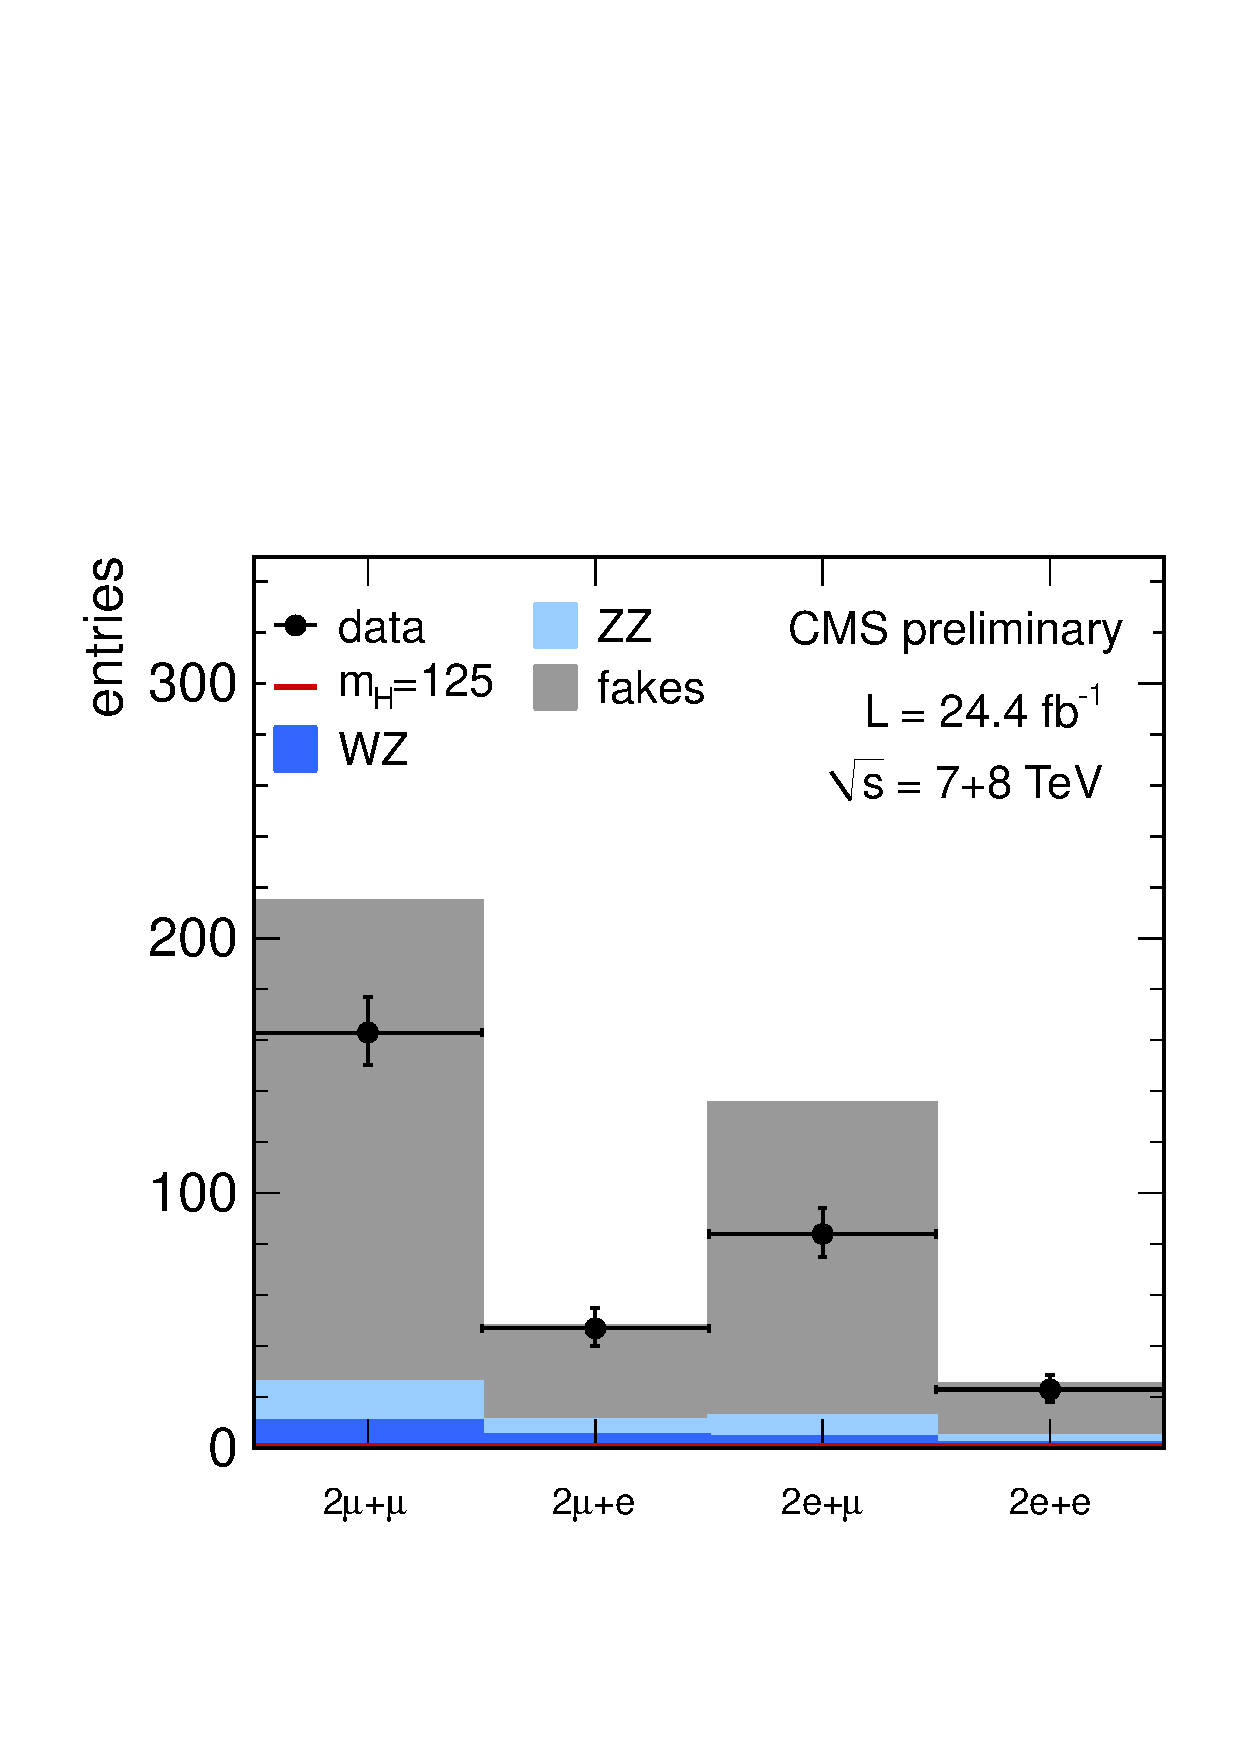
\includegraphics[width=0.45\textwidth]{figures/histo_Zjets15.pdf}
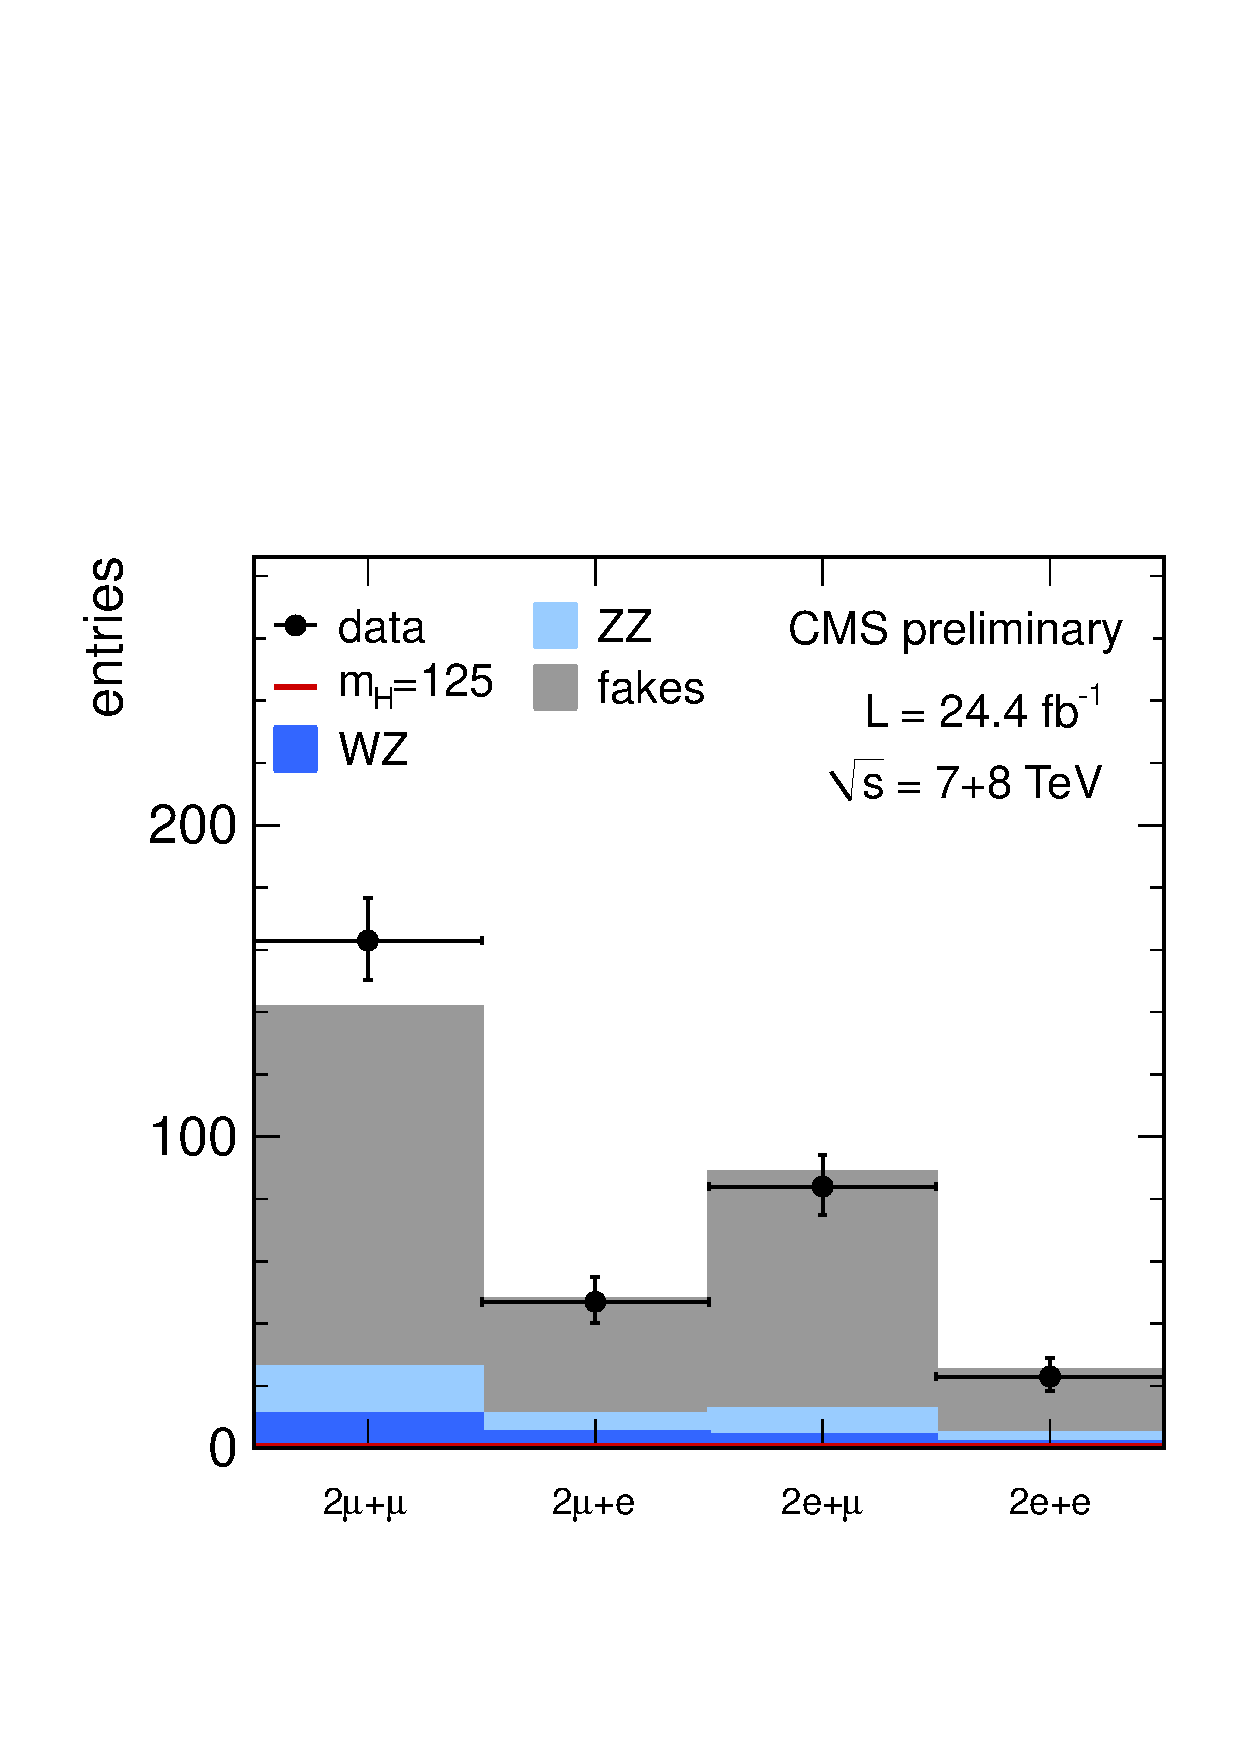
\includegraphics[width=0.45\textwidth]{figures/histo_Zjets30.pdf}
\caption{\label{fig:histo_Zjets} Selected $\Zjets$ events for the different four
lepton categories. The muon fake rates are computed using an away jet $\pt$
greater than 15 $\GeV$ (left) and 30 $\GeV$ (right).}
\end{center}
\end{figure}
